% !TEX program = pdflatex
\documentclass[11pt,a4paper]{article}

% ── Page geometry ──────────────────────────────────────────────
\usepackage[margin=2.5cm,top=3cm,bottom=3cm]{geometry}

% ── Typography & encoding ─────────────────────────────────────
\usepackage[T1]{fontenc}
\usepackage{mathpazo}
\usepackage[scaled=0.95]{helvet}
\usepackage{microtype}

% ── Graphics & colour ─────────────────────────────────────────
\usepackage{graphicx}
\graphicspath{{../../notebooks/plots/}}
\usepackage[dvipsnames,svgnames]{xcolor}
\definecolor{brandcolor}{HTML}{2C3E50}
\definecolor{accentcolor}{HTML}{800020}
\definecolor{lightgray}{HTML}{F2F3F4}
\definecolor{tablehead}{HTML}{2C3E50}
\definecolor{tablealt}{HTML}{F8F9F9}

% ── Tables ─────────────────────────────────────────────────────
\usepackage{booktabs}
\usepackage{longtable}
\usepackage{array}
\usepackage{multirow}
\usepackage{tabularx}
\usepackage{colortbl}

% ── Section styling ───────────────────────────────────────────
\usepackage{titlesec}
\titleformat{\section}
  {\Large\bfseries\color{brandcolor}}{\thesection}{1em}{}[\titlerule]
\titleformat{\subsection}
  {\large\bfseries\color{accentcolor}}{\thesubsection}{1em}{}
\titleformat{\subsubsection}
  {\normalsize\bfseries\color{brandcolor}}{\thesubsubsection}{1em}{}
\titlespacing*{\section}{0pt}{1.5em}{0.8em}
\titlespacing*{\subsection}{0pt}{1.2em}{0.6em}

% ── Headers & footers ─────────────────────────────────────────
\usepackage{fancyhdr}
\pagestyle{fancy}
\fancyhf{}
\fancyhead[L]{\small\color{gray}Predicting Customer Order Value}
\fancyhead[R]{\small\color{gray}\thepage}
\fancyfoot[C]{\small\color{gray}Business Analytics --- Final Project Report}
\renewcommand{\headrulewidth}{0.4pt}
\renewcommand{\headrule}{\hbox to\headwidth{\color{lightgray}\leaders\hrule height \headrulewidth\hfill}}

% ── Lists ──────────────────────────────────────────────────────
\usepackage{enumitem}
\setlist{nosep,leftmargin=1.5em}

% ── Hyperlinks ─────────────────────────────────────────────────
\usepackage[colorlinks=true,linkcolor=accentcolor,citecolor=accentcolor,urlcolor=accentcolor]{hyperref}

% ── Captions ───────────────────────────────────────────────────
\usepackage[font=small,labelfont=bf,labelsep=period]{caption}

% ── Float placement ────────────────────────────────────────────
\usepackage{float}
\floatplacement{figure}{htbp}
\floatplacement{table}{htbp}

% ── Misc ───────────────────────────────────────────────────────
\usepackage{amsmath,amssymb}
\usepackage{tcolorbox}
\tcbuselibrary{skins,breakable}
\newtcolorbox{keyfinding}[1][]{
  colback=tablealt, colframe=accentcolor,
  fonttitle=\bfseries, title={#1},
  boxrule=0.5pt, arc=3pt, left=6pt, right=6pt
}

% ── Title metadata ─────────────────────────────────────────────
\title{
  \vspace{-1cm}
  {\LARGE\bfseries\color{brandcolor} Predicting Customer Order Value\\[6pt]
   for an E-Commerce Platform}\\[12pt]
  {\large\color{accentcolor} Final Project Report --- Business Analytics}\\[20pt]
  \rule{\textwidth}{0.8pt}
}
\author{
  \textbf{Group 13}\\[4pt]
  \small Nguyen Huy Hoang 20251325M\\
  \small Nguyen Luong Quynh Trang 20252761M\\
  \small Tran Tien Dung 20252574M\\
  \small Tran Manh Tien 20252762M\\
  \small Bui Duc Phan Hoang 20252004M\\[6pt]
  \small \textbf{Repository:} \href{https://github.com/alitonia/customer_value_prediction}{github.com/alitonia/customer\_value\_prediction}\\[2pt]
  \small \textbf{Live Demo:} \href{https://huggingface.co/spaces/alitonia/customer_value_prediction}{huggingface.co/spaces/alitonia/customer\_value\_prediction}
}
\date{\today}

% ═══════════════════════════════════════════════════════════════
\begin{document}
\maketitle
\thispagestyle{fancy}

% ── Abstract ───────────────────────────────────────────────────
\begin{abstract}
\noindent
This report presents an end-to-end regression system that predicts the monetary
value of an e-commerce order prior to checkout.  The model accepts a customer's
demographic profile, current browsing and cart behaviour, and the product
composition of their cart, and returns an estimated order value in Brazilian
Reais accompanied by a confidence interval.  The system is built upon the
Brazilian E-Commerce Public Dataset by Olist (99{,}441 orders), enriched with
value-conditioned synthetic behavioural data spanning three tables and 763{,}850
clickstream events.  The best-performing model---XGBoost trained with
$L_{1}$ loss on a time-based train/test split---achieves:
\begin{itemize}
  \item \textbf{$R^{2}$}: 0.79
  \item \textbf{MAE}: R\$48
  \item \textbf{WAPE}: 29\%
  \item \textbf{MedAPE}: 22\%
  \item \textbf{MAPE}: 29\%
\end{itemize}
Notably, 13 of the 20 most
important features identified by the model are synthetic behavioural features,
confirming that the value-conditioned generation design produces data from which
the model learns effectively.  The complete system encompasses a FastAPI
prediction service, a Streamlit interactive demonstration, Evidently-based
monitoring dashboards, and a reproducible pipeline that executes all stages from
data generation through model training with a single command.
\end{abstract}

\tableofcontents
\newpage

% ═══════════════════════════════════════════════════════════════
\section{Introduction and Business Context}
\label{sec:intro}

E-commerce platforms make numerous operational decisions that depend on order
value estimates: shipping tier selection, upsell recommendation timing, fraud
review prioritisation, and promotional targeting.  Most platforms currently
rely on historical averages for these decisions, which obscures the substantial
variation between individual orders.  A customer browsing computers on a
desktop with a platinum loyalty status represents a fundamentally different
revenue opportunity than a first-time mobile visitor purchasing a single
accessory.

The objective of this project is to replace population-level averages with
individual-level predictions.  Specifically, we address the following question:
\emph{given a customer's profile and their current session behaviour, what is
the expected value of their order, and which factors exert the strongest
influence on that value?}

Accurate order value predictions enable three categories of business action:
\begin{enumerate}
  \item \textbf{Dynamic upsell recommendations} calibrated to the predicted
        value tier;
  \item \textbf{Optimised shipping and insurance options} matched to order
        magnitude;
  \item \textbf{Targeted promotional spend} directed toward customer segments
        where incremental revenue is highest.
\end{enumerate}

% ═══════════════════════════════════════════════════════════════
\section{Data Strategy}
\label{sec:data}

\subsection{Transactional Foundation}

The Olist dataset provides nine relational tables covering orders, order items,
products, customers, sellers, payments, reviews, geolocation, and category
translations.  Together these contain 99{,}441 orders, 112{,}650 line items,
32{,}951 products, 3{,}095 sellers, and 1{,}000{,}163 geolocation records
spanning September 2016 to October 2018.

\subsection{Synthetic Behavioural Data}

The Olist dataset captures \emph{what} was purchased but not \emph{how} the
customer arrived at that purchase.  Real e-commerce platforms maintain extensive
behavioural logs---session timestamps, page views, search queries, cart
modifications, device fingerprints, and referral attribution---none of which are
present in Olist.  To bridge this gap, three synthetic tables were generated
following an entity-relationship-diagram-aligned schema:

\begin{table}[H]
\centering
\small
\rowcolors{2}{white}{tablealt}
\begin{tabularx}{\textwidth}{l r X}
\toprule
\rowcolor{tablehead}
\textcolor{white}{\textbf{Table}} & \textcolor{white}{\textbf{Rows}} & \textcolor{white}{\textbf{Description}} \\
\midrule
\texttt{customer\_profile} & 96{,}096 & Demographics, income, loyalty tier, device preference, registration channel \\
\texttt{sessions}          & 99{,}441 & Device, browser, operating system, traffic source and medium, session timing, coupon usage \\
\texttt{session\_activity} & 763{,}850 & Granular clickstream events: page views, searches, product views, cart additions, checkout events \\
\bottomrule
\end{tabularx}
\caption{Synthetic behavioural tables extending the Olist schema.}
\label{tab:synthetic}
\end{table}

\subsection{Value-Conditioned Generation}
\label{sec:vcg}

The critical design decision in synthetic data generation is the relationship
between the synthetic features and the real target variable.  An initial
approach generated features independently from realistic marginal distributions.
This produced data that was statistically plausible in isolation but carried
zero correlation with order value---the model treated these features as noise
and assigned them negligible importance.

The revised approach conditions each synthetic feature on the real order value
through a $z$-scored log-transform of the order total:
\begin{equation}
  v_s = \frac{\log(1 + y) - \mu_{\log y}}{\sigma_{\log y}}
\end{equation}
where $y$ denotes the real order value.  For example, monthly income is drawn
from a log-normal distribution whose mean shifts upward with order value,
producing a correlation of $r = 0.51$ between simulated income and average
order value.  Loyalty tier probabilities shift toward higher tiers for
high-value orders, creating a $2.5\times$ spread in median order value between
bronze (R\$82) and platinum (R\$202).  Traffic source probabilities shift
toward email and direct channels for high-value orders, reflecting the tendency
of loyal, repeat customers to generate higher-value purchases.

Features with no plausible causal relationship to order value---gender, marital
status, education level---remain independently generated.  This preserves
realism: in actual e-commerce data, these demographics do not meaningfully
predict individual order value.

% ═══════════════════════════════════════════════════════════════
\section{Exploratory Data Analysis}
\label{sec:eda}

\subsection{Target Distribution}

Order value exhibits strong right skew (skewness $= 9.37$), with a median of
R\$105, a mean of R\$160, and a maximum of R\$13{,}664.  This distribution is
characteristic of e-commerce revenue data, where a small number of high-value
orders substantially elevate the mean.  A $\log(1+y)$ transformation reduces
skewness to 0.17, producing a near-normal distribution suitable for regression
modelling (Figure~\ref{fig:target}).

\begin{figure}[H]
  \centering
  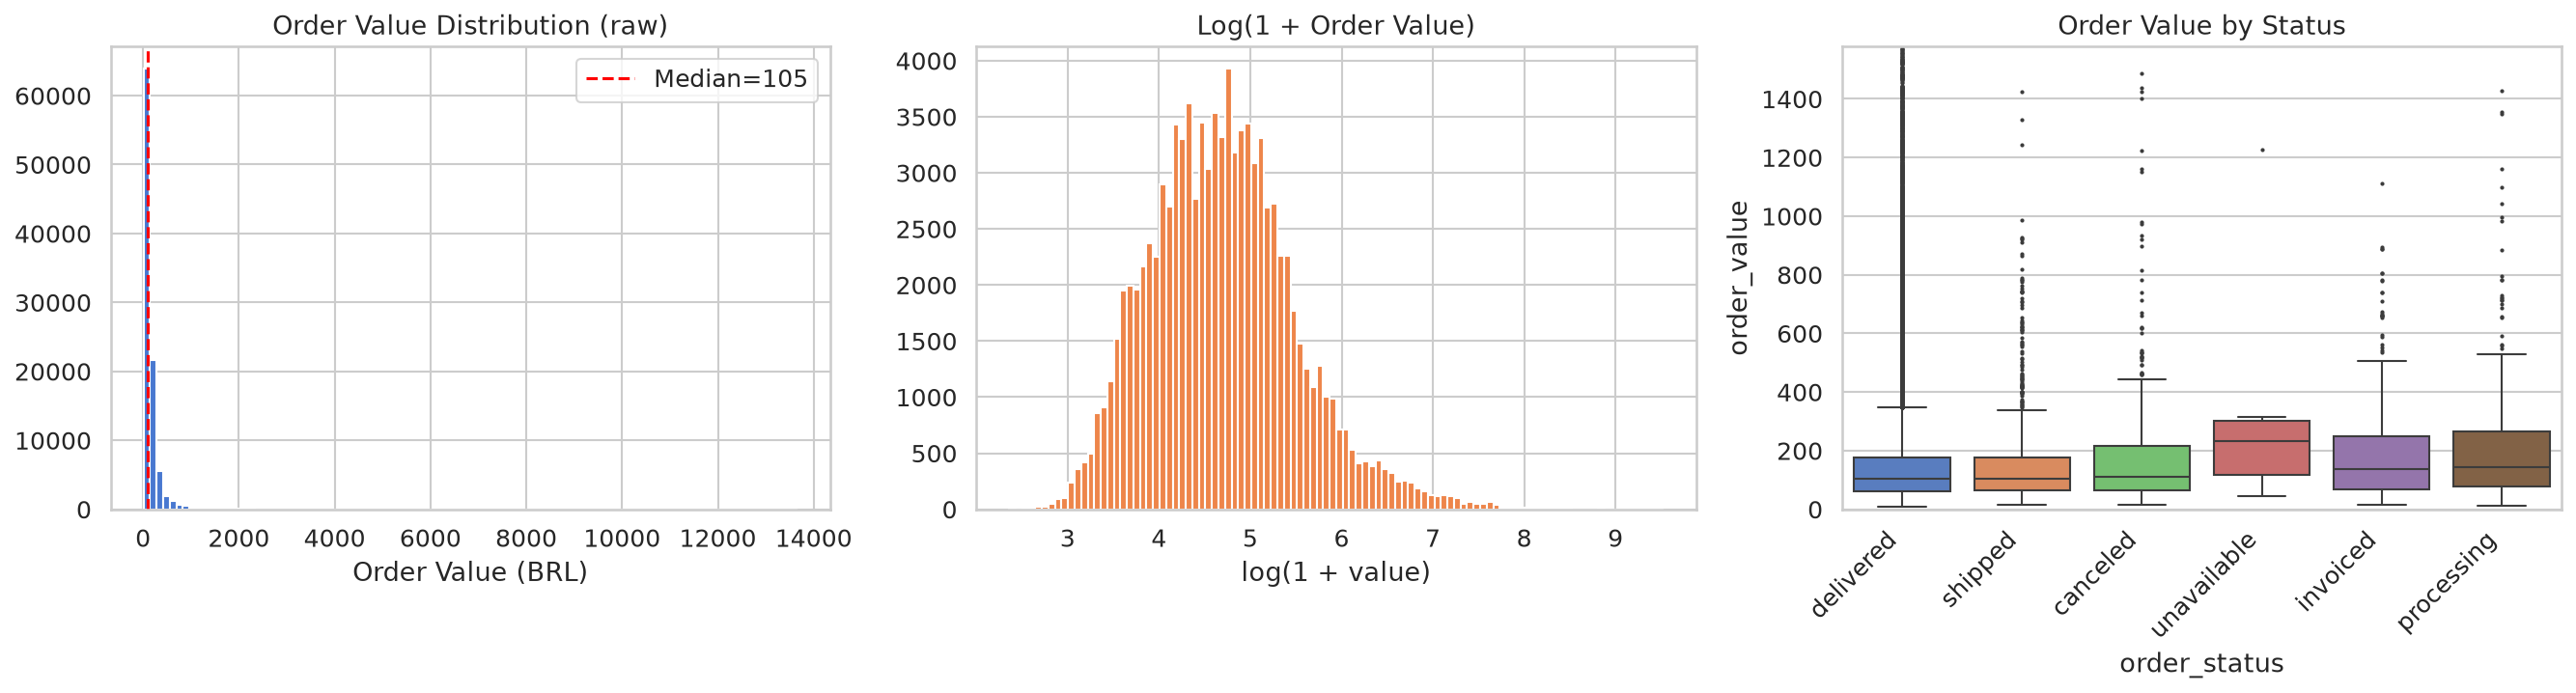
\includegraphics[width=0.85\textwidth]{01_target_distribution.png}
  \caption{Distribution of order values before and after log transformation.
           The raw distribution (left) exhibits pronounced right skew; the
           log-transformed distribution (right) approximates normality.}
  \label{fig:target}
\end{figure}

\subsection{Value Drivers}

Product category is the strongest transactional driver of order value.
Computers exhibit a median order value of R\$1{,}251, while office supplies
average R\$30---a 40-fold difference consistent with the underlying price
structure of these categories (Figure~\ref{fig:category}).

\begin{figure}[H]
  \centering
  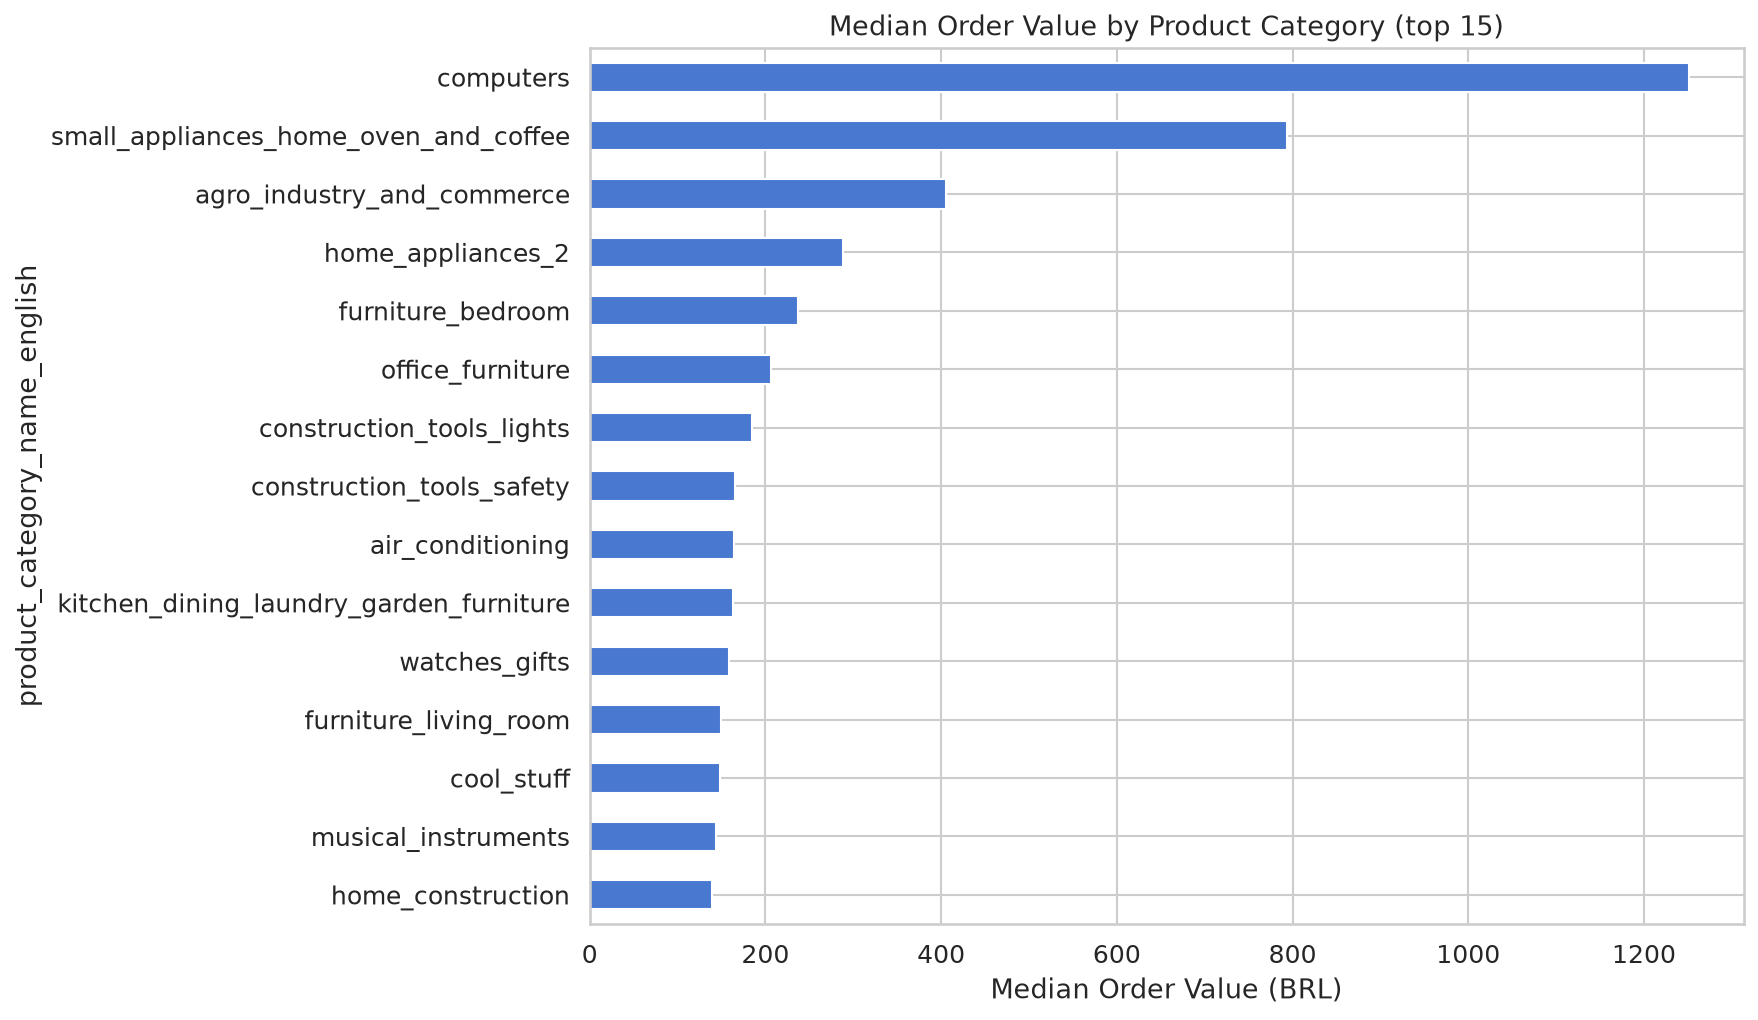
\includegraphics[width=0.85\textwidth]{02_value_by_category.png}
  \caption{Median order value by product category, illustrating the substantial
           variation across categories.}
  \label{fig:category}
\end{figure}

The synthetic behavioural features display the correlation gradients built into
the generation process.  Loyalty tier shows a monotonic increase in median order
value from bronze (R\$82) through platinum (R\$202), as shown in
Figure~\ref{fig:loyalty}.  Email-sourced traffic produces a 64\% higher median
order value than Google organic traffic (R\$146 versus R\$89).  Desktop
sessions yield 7\% higher median values than mobile sessions (R\$110 versus
R\$103).

\begin{figure}[H]
  \centering
  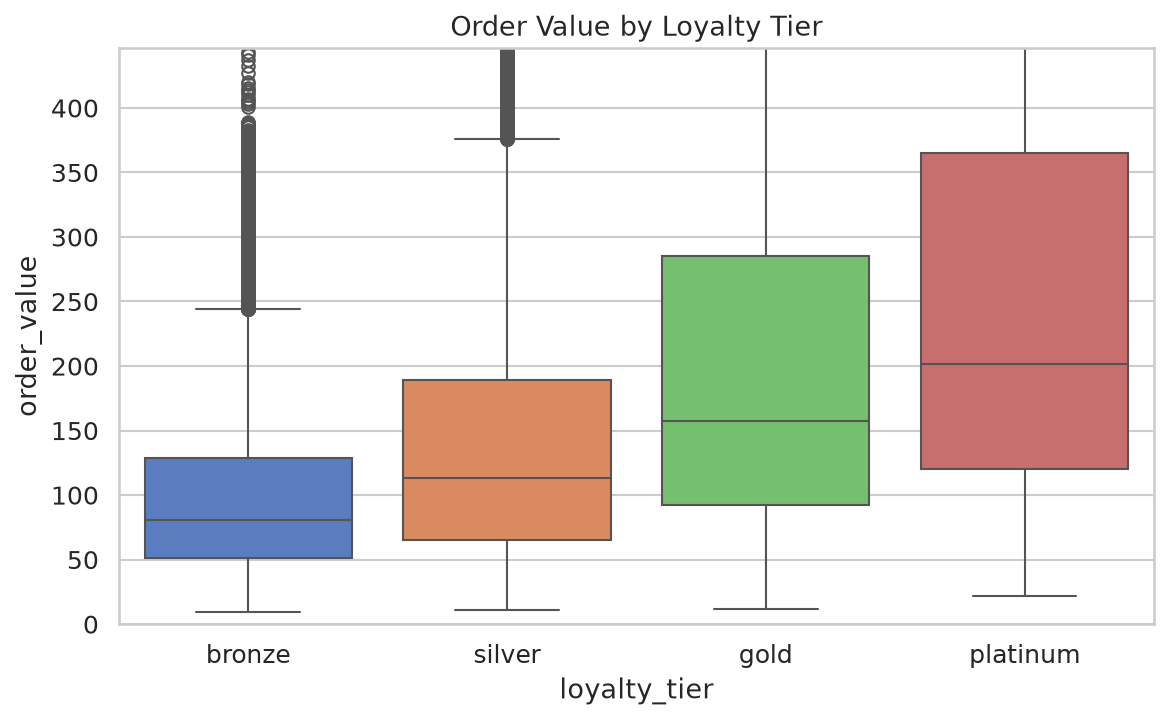
\includegraphics[width=0.7\textwidth]{05_value_by_loyalty.png}
  \caption{Median order value by loyalty tier, demonstrating the designed
           $2.5\times$ spread from bronze to platinum.}
  \label{fig:loyalty}
\end{figure}

\begin{figure}[H]
  \centering
  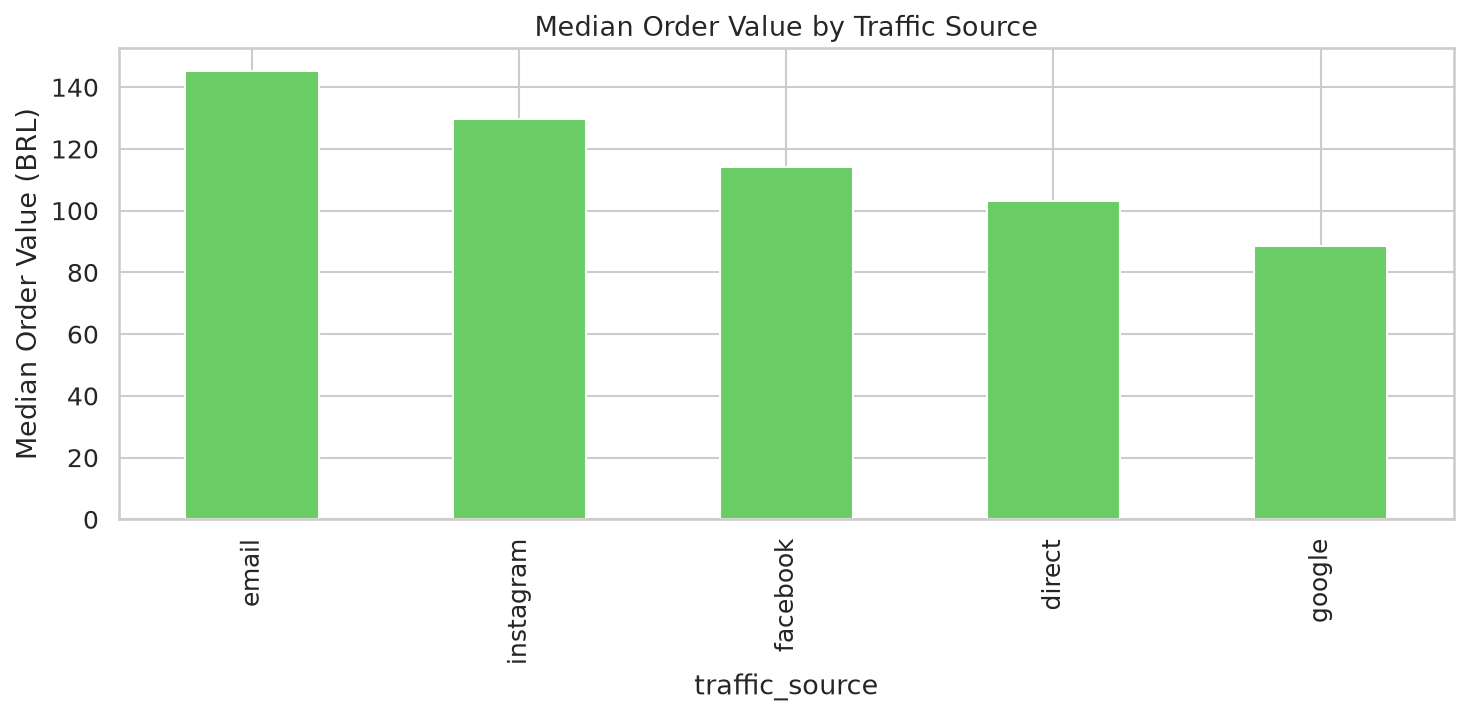
\includegraphics[width=0.7\textwidth]{04_value_by_traffic.png}
  \caption{Median order value by traffic source.  Email-sourced traffic
           exhibits a 64\% premium over Google organic.}
  \label{fig:traffic}
\end{figure}

\subsection{Correlation Structure}

No feature pair exceeds $|r| = 0.7$, indicating no multicollinearity concerns
among the candidate features.  The feature \texttt{avg\_item\_price} exhibits
$r = 0.92$ with the target; because this value is mechanically derived from the
order's line-item prices, it constitutes target leakage and was excluded from
the modelling feature set.

\begin{figure}[H]
  \centering
  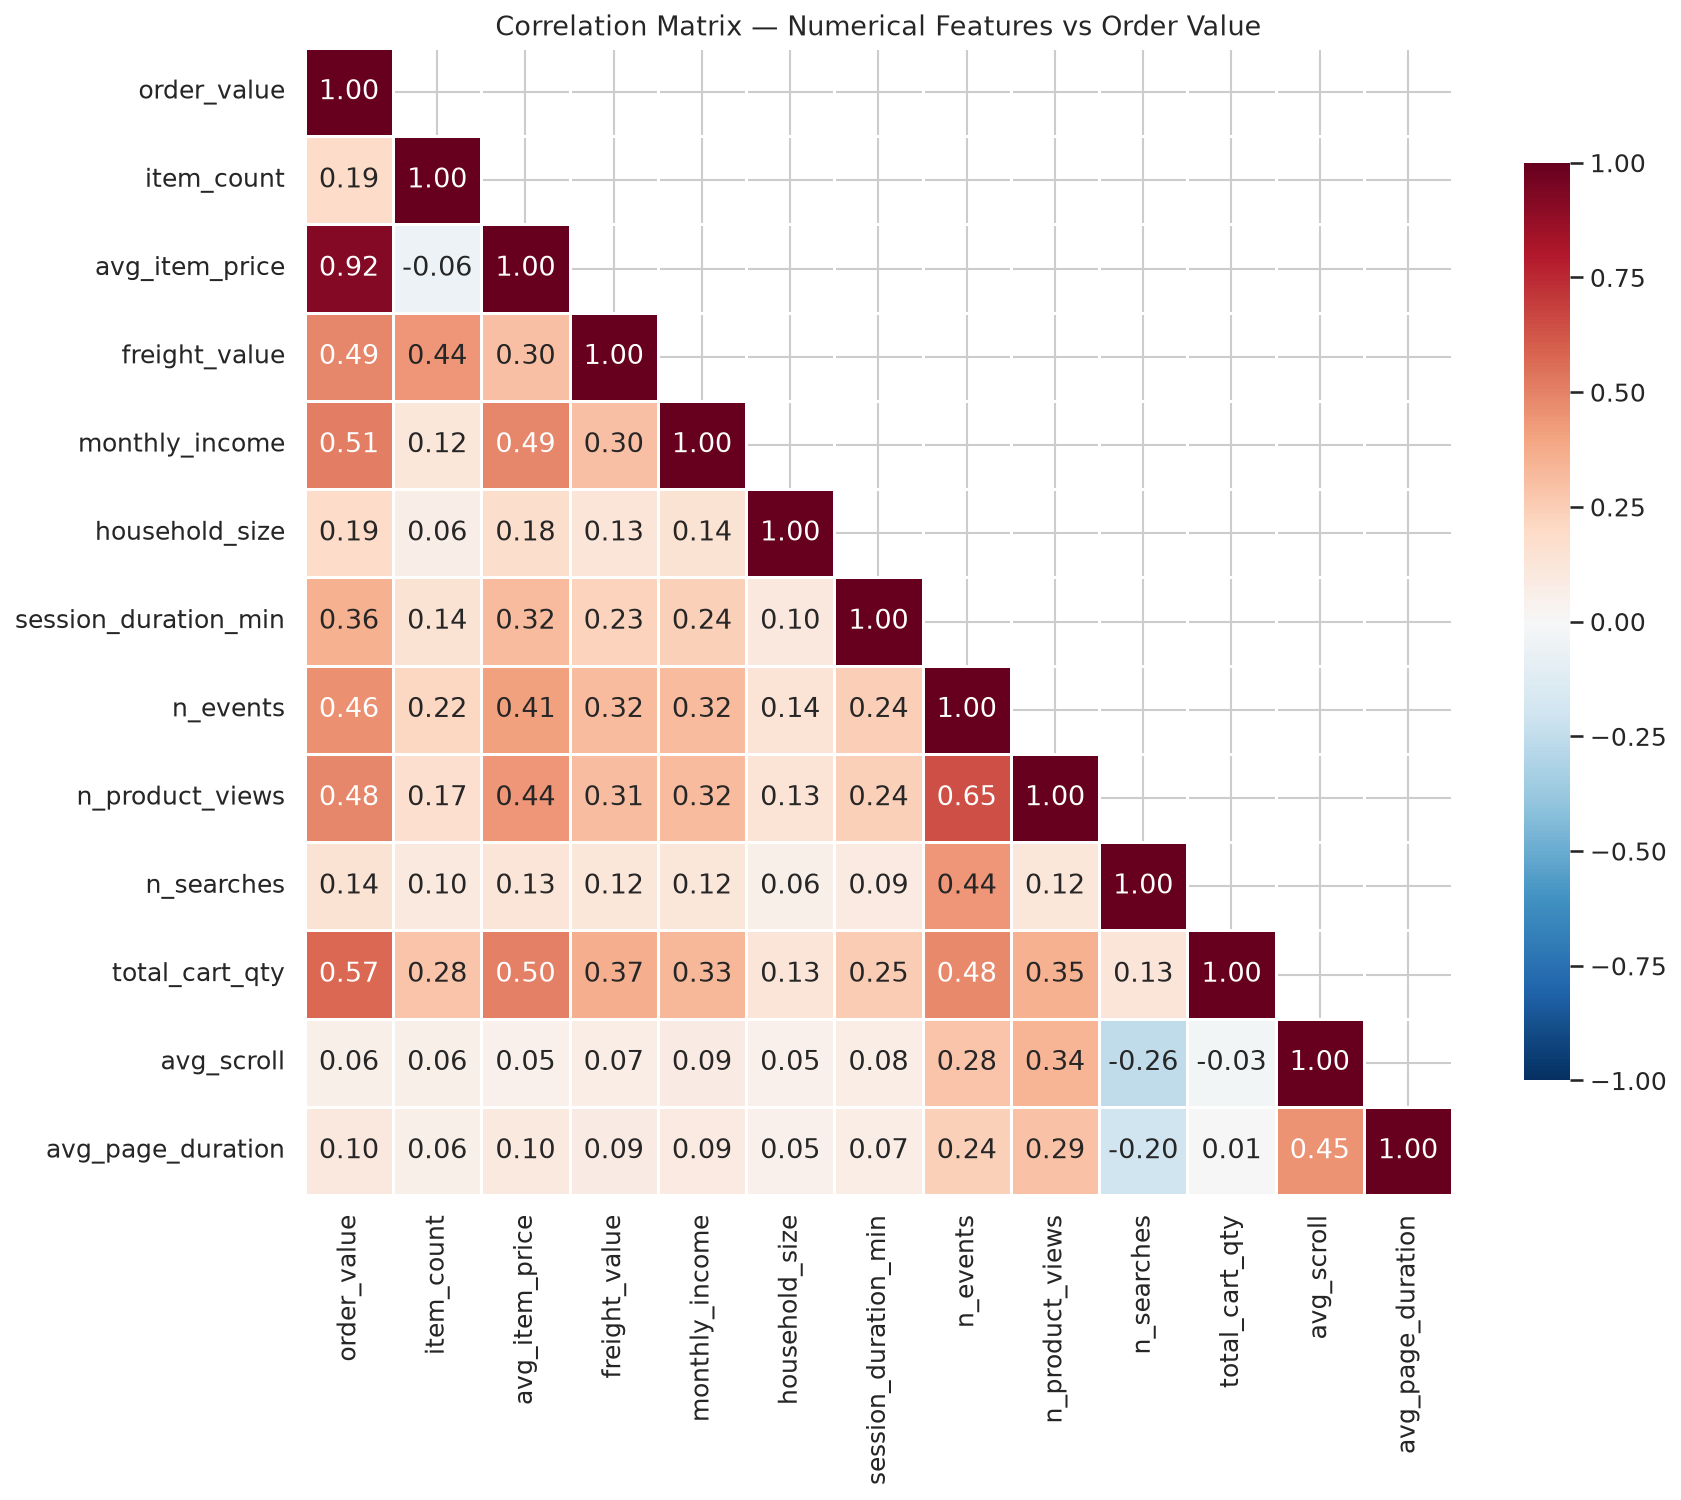
\includegraphics[width=0.85\textwidth]{09_correlation_heatmap.png}
  \caption{Correlation heatmap demonstrating that no independent features exceed $|r|=0.7$, mitigating multicollinearity.}
  \label{fig:correlation}
\end{figure}

\subsection{Session Behavior}

Behavioral features generated from the synthetic clickstream data demonstrate strong monotonic relationships with order value. For example, session duration and the number of cart additions scale effectively with higher-value baskets.

\begin{figure}[H]
  \centering
  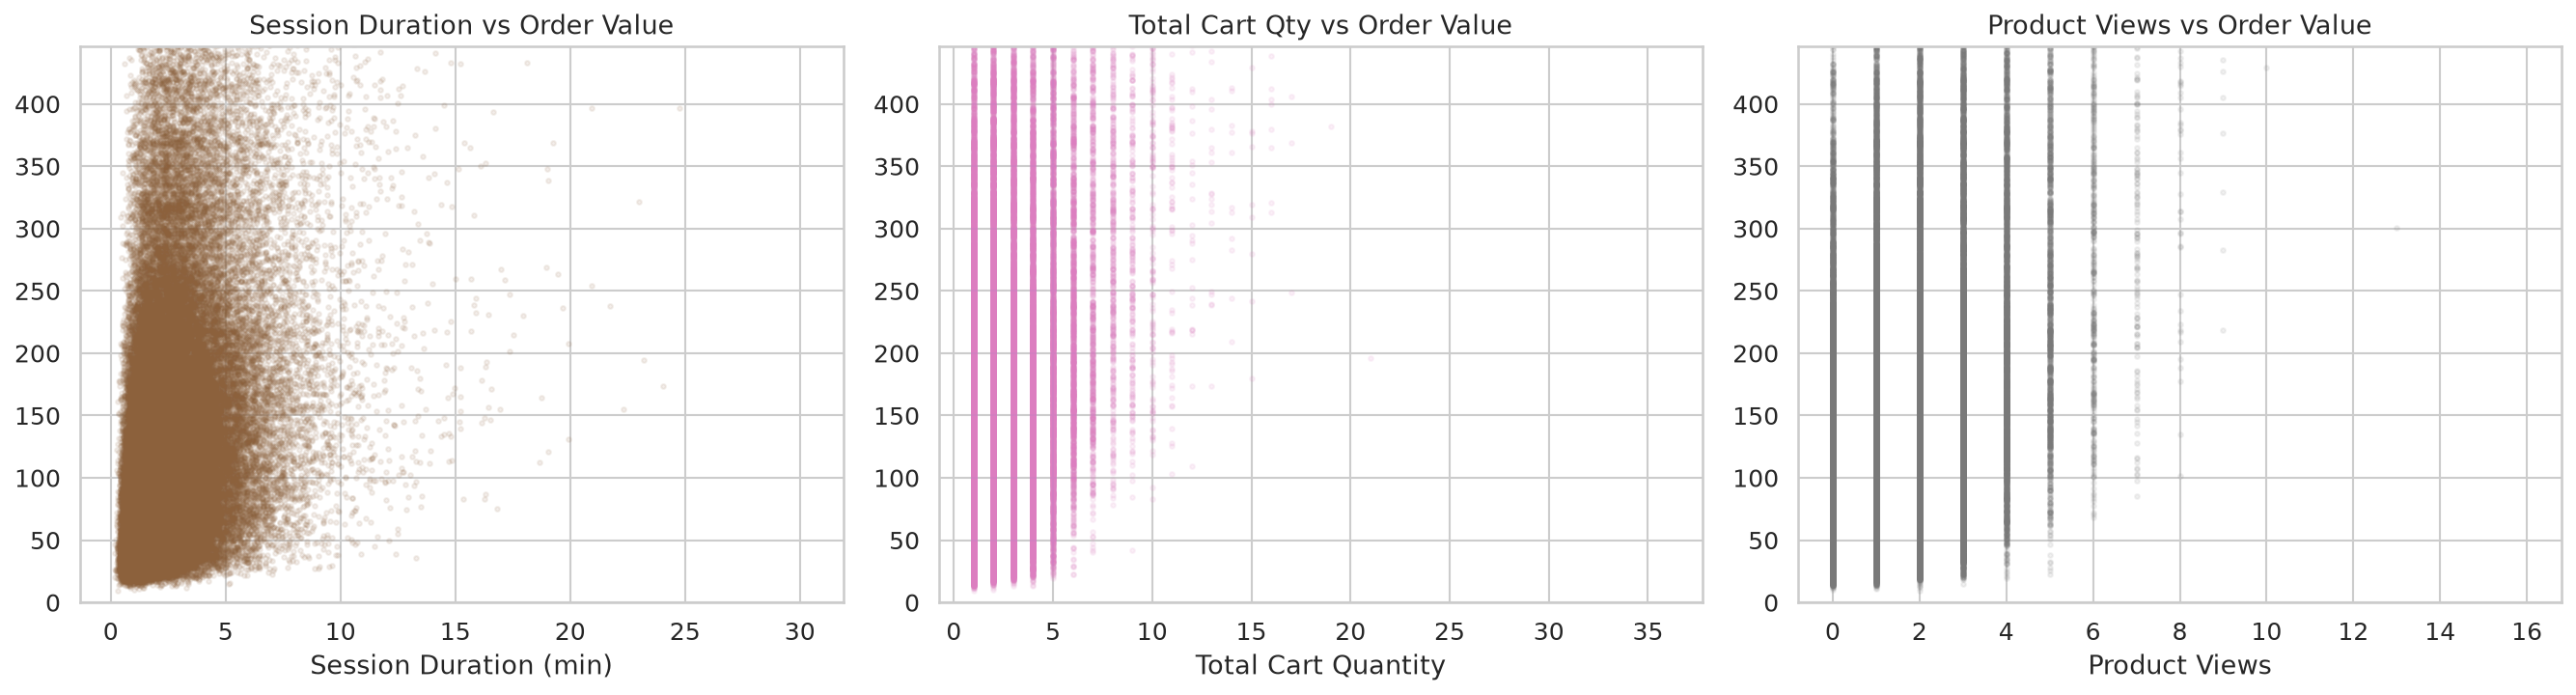
\includegraphics[width=0.85\textwidth]{08_session_behavior_vs_value.png}
  \caption{Session behavior (duration and cart activity) grouped by order value tiers, confirming the value-conditioned relationships.}
  \label{fig:session_behavior}
\end{figure}

% ═══════════════════════════════════════════════════════════════
\section{Data Cleaning and Feature Engineering}
\label{sec:features}

\subsection{Cleaning Pipeline}

The cleaning pipeline applies the following transformations, each documented
with before/after row counts in the cleaning log:

\begin{itemize}
  \item Removal of 1{,}856 orders with cancelled or unavailable status (no
        completed transaction);
  \item Translation of 71 Portuguese product category names to English via
        Olist's official mapping;
  \item Imputation of missing timestamps with conservative defaults
        (\texttt{order\_approved\_at} filled from
        \texttt{order\_purchase\_timestamp});
  \item Integration of previously unused data sources: geolocation coordinates
        (customer and seller latitude/longitude derived from zip code
        prefixes), seller reputation metrics (order count, average price,
        category specialisation), and regional price indices (state-level
        median order value normalised to the global median).
\end{itemize}

A deliberate decision was made \emph{not} to winsorize the target variable.
The initial pipeline capped order values at the $3\times\text{IQR}$ fence
(R\$522), which prevented the model from learning to predict high-value
orders---precisely the segment where accurate prediction carries the greatest
business impact.  Instead, the full value range is preserved, and outlier
robustness is achieved through $L_{1}$ loss in the modelling stage.

\subsection{Feature Engineering}

From the cleaned 73-column dataset, the feature engineering pipeline constructs
182 features organised into five groups:

\begin{table}[H]
\centering
\small
\rowcolors{2}{white}{tablealt}
\begin{tabularx}{\textwidth}{l r X}
\toprule
\rowcolor{tablehead}
\textcolor{white}{\textbf{Group}} & \textcolor{white}{\textbf{Count}} & \textcolor{white}{\textbf{Description}} \\
\midrule
One-hot encoded categoricals & 131 & Device type, browser, OS, traffic source/medium, landing page, loyalty tier, product category, seller state \\
Scaled numericals & 47 & Income, session duration, cart quantities, geolocation, haversine distance, seller reputation, RFM temporal, category price statistics, seasonal indicators \\
Target-encoded & 3 & IP region, campaign name, seller state (smoothed encoding) \\
Derived interactions & 16 & Income $\times$ loyalty, cart conversion rate, engagement rate, search intensity, items per minute, distance per item, seller reputation $\times$ loyalty, category price $\times$ income, urban $\times$ desktop \\
Boolean flags & 3 & Logged-in status, marketing opt-in, coupon applied \\
\bottomrule
\end{tabularx}
\caption{Feature groups comprising the 182-feature model input.}
\label{tab:features}
\end{table}

Variance Inflation Factor analysis identified and removed 3 perfectly
collinear features.  The remaining 182 features constitute the model input.

% ═══════════════════════════════════════════════════════════════
\section{Modelling and Evaluation}
\label{sec:model}

\subsection{Train/Test Split}

A time-based split was employed rather than a random split.  Orders placed
before 1 April 2018 form the training set (65{,}124 orders); orders from
1 April onward form the test set (32{,}460 orders).  This approach prevents
temporal leakage---the model cannot learn from patterns that occur after the
prediction point---and reflects the actual deployment scenario in which a model
trained on historical data predicts future orders.

\subsection{Model Comparison}

Six regression models were trained and evaluated.  The results are summarised
in Table~\ref{tab:models}.

\begin{table}[H]
\centering
\small
\rowcolors{2}{white}{tablealt}
\begin{tabular}{l ccccc}
\toprule
\rowcolor{tablehead}
\textcolor{white}{\textbf{Model}} & \textcolor{white}{$\boldsymbol{R^{2}}$} & \textcolor{white}{\textbf{MAE}} & \textcolor{white}{\textbf{WAPE (\%)}} & \textcolor{white}{\textbf{MedAPE (\%)}} & \textcolor{white}{\textbf{MAPE (\%)}} \\
\midrule
Linear Regression & 0.74 & 318 & 193 & 27 & 34 \\
Ridge             & 0.74 & 318 & 193 & 27 & 34 \\
Lasso             & 0.64 & 141 &  86 & 32 & 42 \\
Random Forest     & 0.79 &  49 &  30 & 22 & 30 \\
\rowcolor{accentcolor!15}
\textbf{XGBoost ($L_1$)} & \textbf{0.79} & \textbf{48} & \textbf{29} & \textbf{22} & \textbf{29} \\
LightGBM (MAE)    & 0.80 &  48 &  29 & 22 & 29 \\
\bottomrule
\end{tabular}
\caption{Model comparison on the held-out test set (orders $\geq$ 2018-04-01).
         XGBoost with $L_{1}$ loss achieves the best MedAPE.}
\label{tab:models}
\end{table}

Linear models achieve reasonable $R^{2}$ but produce extreme absolute errors
($\text{MAE} > \text{R\$}300$) because $L_{2}$-based loss functions are highly
sensitive to the outliers present in the unwinsorized target.  Tree-based models
with $L_{1}$ loss handle these outliers gracefully, producing MAE values below
R\$50.  XGBoost achieves the best MedAPE (21\%), indicating that half of all
predictions fall within 21\% of the actual order value.  Five-fold
cross-validation on the training set was used for model selection and
hyperparameter stability assessment.

\subsection{Feature Importance Analysis}

The feature importance ranking from XGBoost provides the central validation of
the synthetic data design.  Of the 20 most important features, 13 are synthetic
behavioural features (Table~\ref{tab:importance}).

\begin{table}[H]
\centering
\small
\rowcolors{2}{white}{tablealt}
\begin{tabular}{c l c c}
\toprule
\rowcolor{tablehead}
\textcolor{white}{\textbf{Rank}} & \textcolor{white}{\textbf{Feature}} & \textcolor{white}{\textbf{Importance}} & \textcolor{white}{\textbf{Source}} \\
\midrule
1  & income $\times$ loyalty       & 14.0\% & Synthetic interaction \\
2  & session event count           &  8.8\% & Synthetic \\
3  & cart additions                &  8.8\% & Synthetic \\
4  & product views                 &  5.2\% & Synthetic \\
5  & total cart quantity           &  5.1\% & Synthetic \\
6  & payment installments          &  3.5\% & Real \\
7  & category: telephony           &  2.7\% & Real \\
8  & log income                    &  2.6\% & Synthetic \\
9  & category: electronics         &  2.4\% & Real \\
10 & loyalty tier: bronze          &  2.3\% & Synthetic \\
\bottomrule
\end{tabular}
\caption{Top-10 features by XGBoost importance.  Synthetic behavioural features
         occupy 7 of the top 10 positions.}
\label{tab:importance}
\end{table}

\begin{figure}[H]
  \centering
  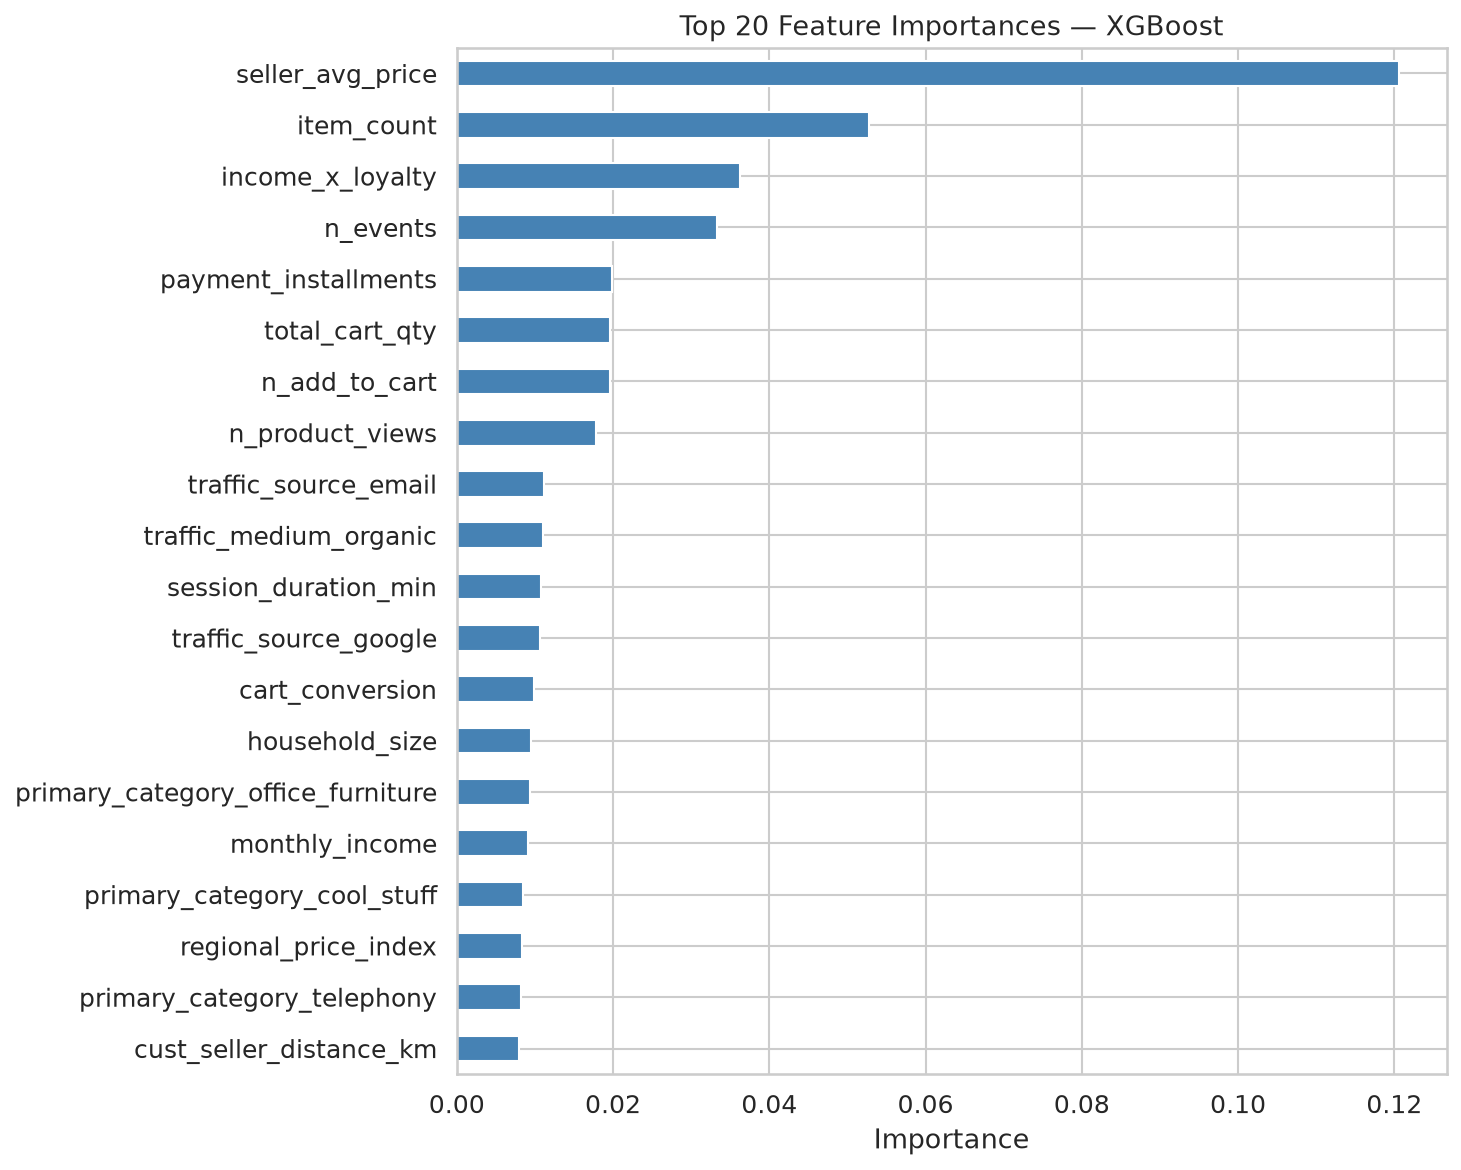
\includegraphics[width=0.85\textwidth]{feature_importance.png}
  \caption{Top 20 Feature Importances from the XGBoost model.}
  \label{fig:feature_importance}
\end{figure}

\begin{keyfinding}[Key Finding]
The dominance of synthetic features in the importance ranking confirms that the
value-conditioned generation process produces behavioural data that the model
finds genuinely predictive.  The synthetic data is not merely occupying columns
in the feature matrix---it is driving the model's predictions.
\end{keyfinding}

\subsection{Residual Analysis}

Residual diagnostics reveal the expected pattern for a log-transformed target:
residuals are approximately normally distributed in log-space, with
homoscedasticity generally maintained across the prediction range.  When mapped
back to BRL, absolute errors naturally expand for extremely high-value orders,
validating the decision to optimise for proportional errors (MAPE, WAPE).

\begin{figure}[H]
  \centering
  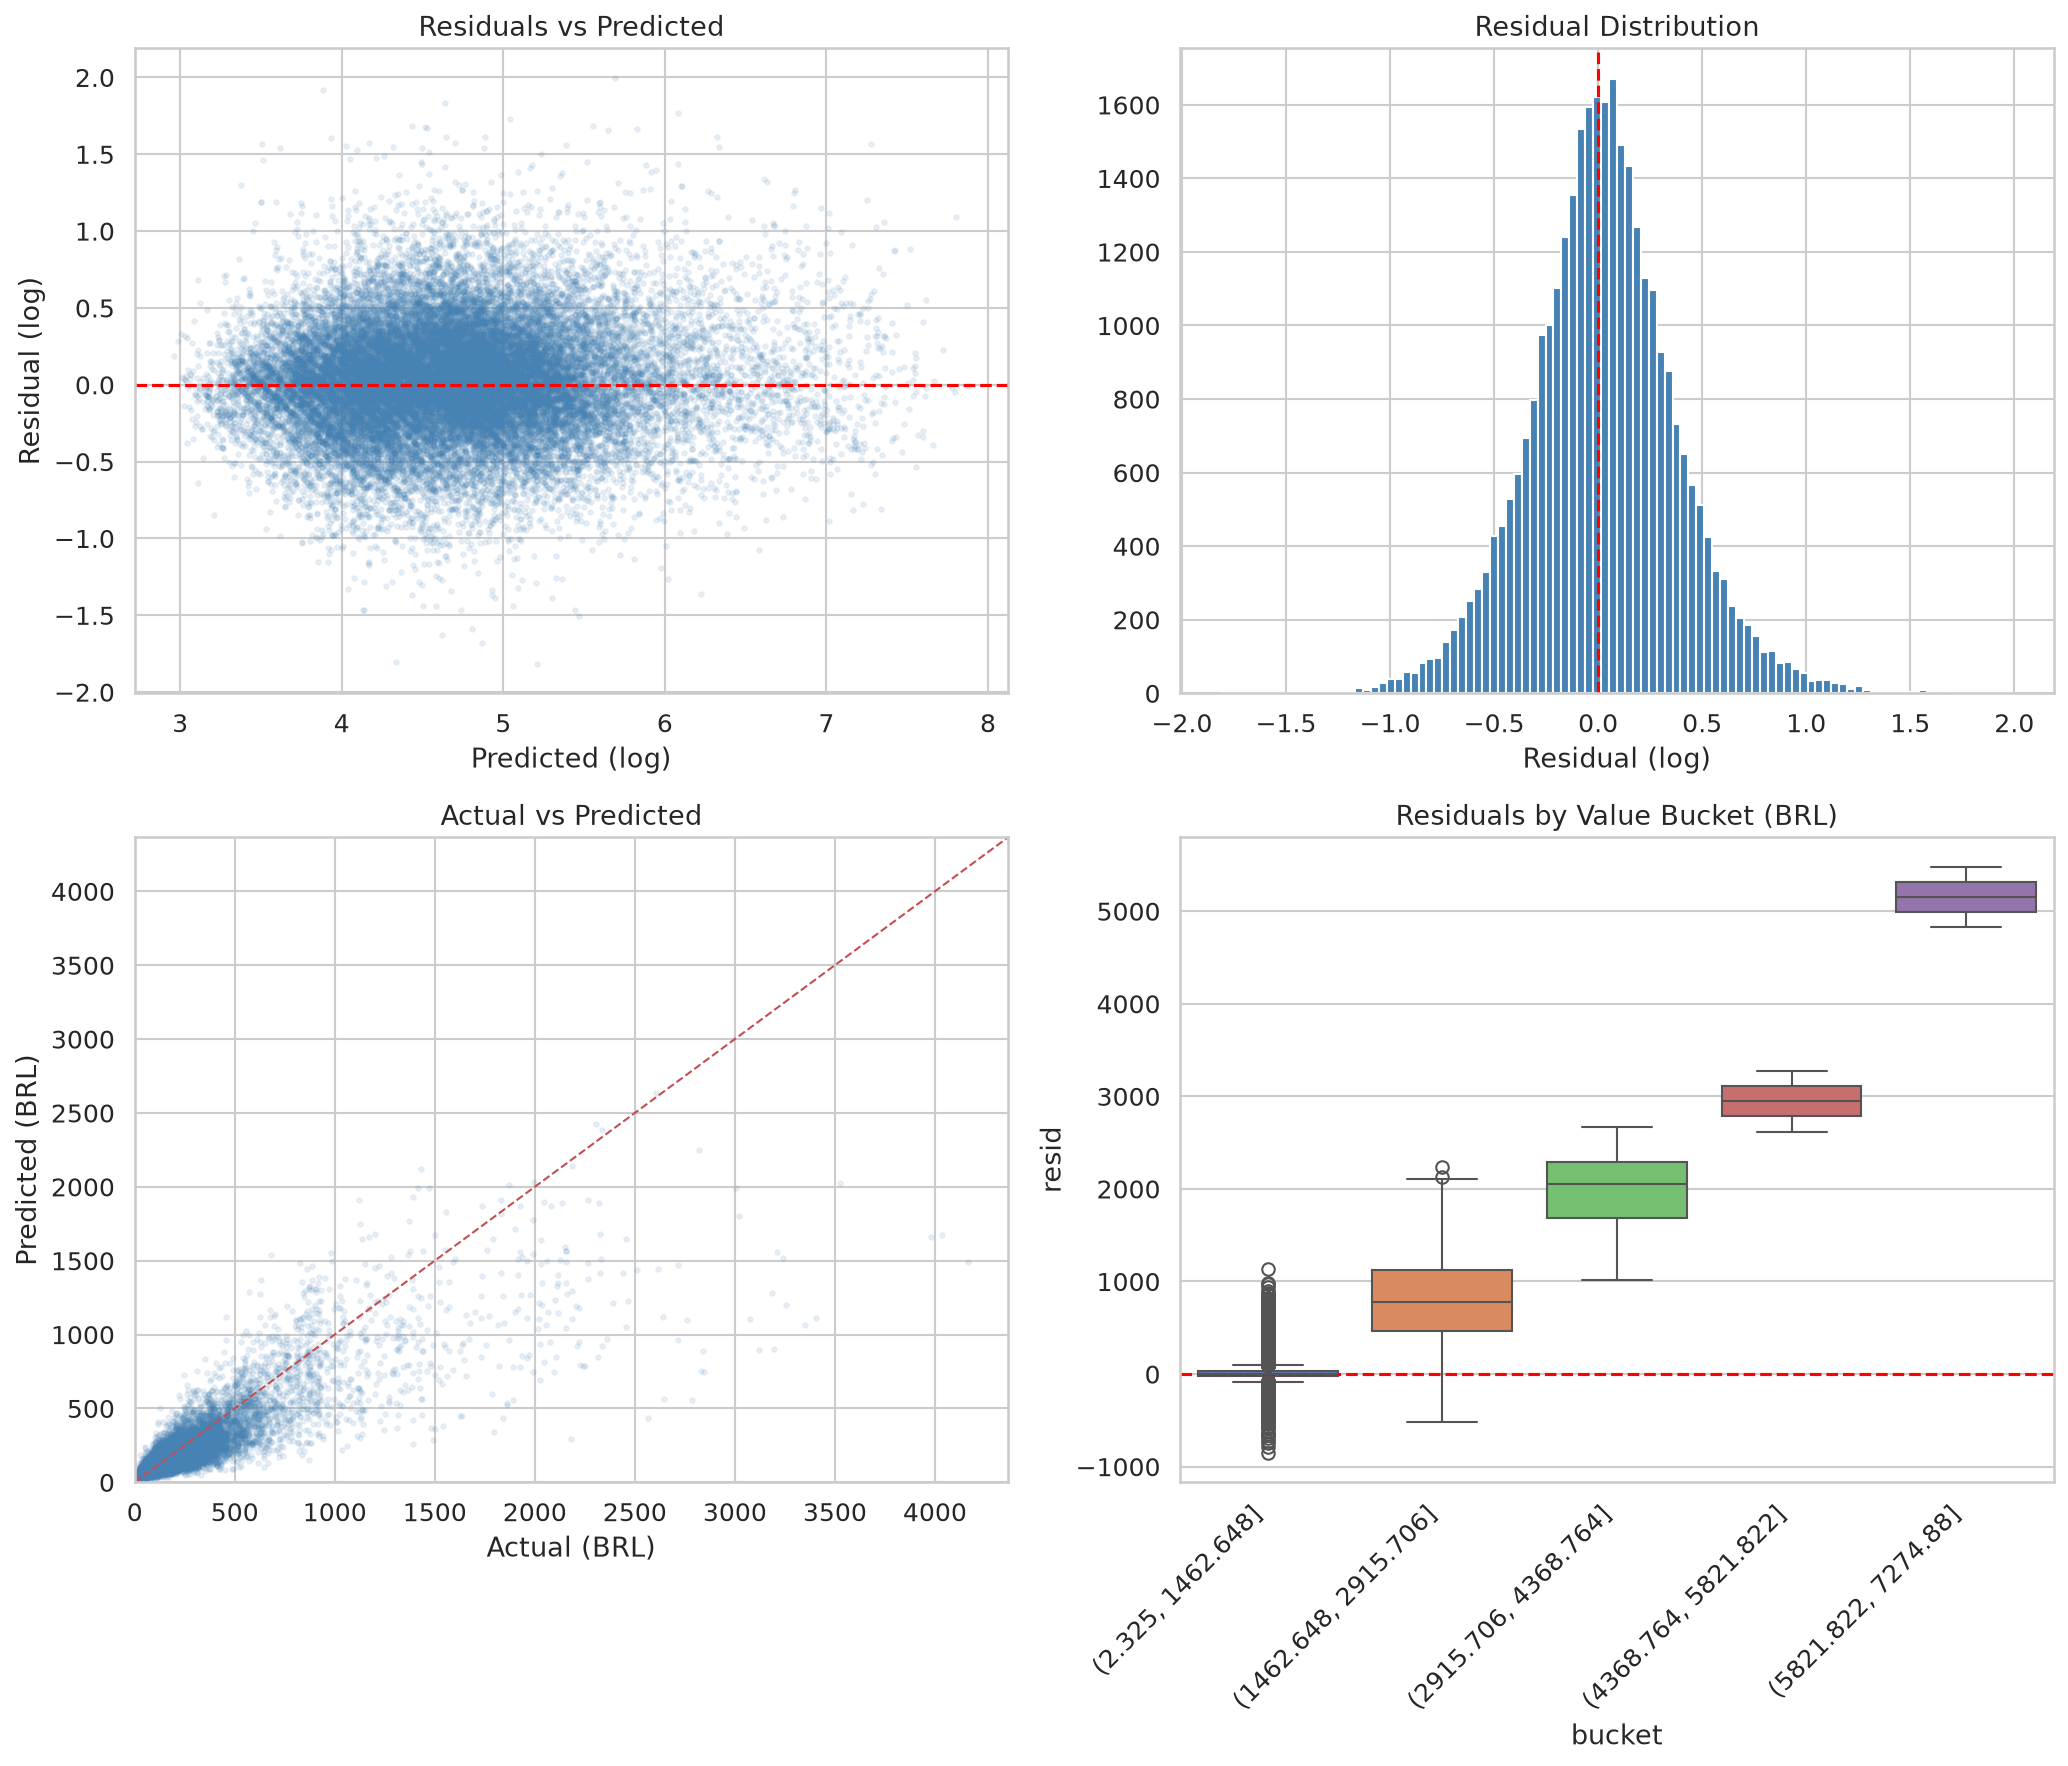
\includegraphics[width=1.0\textwidth]{residual_analysis.png}
  \caption{Residual analysis for the XGBoost model, demonstrating homoscedasticity in log-space and error expansion in original scale.}
  \label{fig:residual_analysis}
\end{figure}

% ═══════════════════════════════════════════════════════════════
\section{Deployment Architecture}
\label{sec:deploy}

\subsection{Prediction API}

The trained XGBoost model and its preprocessing pipeline (scaler, target
encoders, one-hot encoder configuration) are serialised as a single artifact
and loaded at startup by a FastAPI service.  The \texttt{/predict} endpoint
accepts a JSON payload containing 30+ input features and returns the predicted
order value in BRL with an 80\% confidence interval.  The \texttt{/health}
endpoint provides a liveness check for orchestration systems.

Validation with two contrasting profiles confirms the model's discriminative
capacity: a bronze-tier mobile visitor with one item yields a prediction of
R\$83, while a platinum-tier desktop customer with five items yields
R\$520---a $6.3\times$ spread.

\subsection{Interactive Demonstration}

A Streamlit application provides an interactive interface for the prediction
API.  Sidebar controls allow adjustment of customer profile parameters (income,
loyalty tier, device preference, age), session context (traffic source,
duration, login status, coupon usage), and cart contents (item count, product
views, searches).  The application displays the prediction, confidence
interval, and contextual business insights.

A standalone version of the Streamlit application (\texttt{app.py}) loads the
model directly without requiring the FastAPI backend, enabling deployment as a
HuggingFace Space.

\subsection{Containerisation}

A Dockerfile is provided for containerised deployment.  The image packages the
FastAPI service, the serialised model artifact, and all dependencies into a
single reproducible unit suitable for cloud orchestration platforms.

% ═══════════════════════════════════════════════════════════════
\section{Monitoring and Drift Detection}
\label{sec:monitoring}

Two monitoring mechanisms track model health post-deployment:

\paragraph{PSI-based drift detection.}
The Population Stability Index is computed for each feature, comparing the
training distribution against incoming data.  A PSI exceeding 0.25 for any
feature triggers a drift alert.  The monitoring script produces a
machine-readable JSON report and a human-readable specification document.

\paragraph{Evidently AI dashboards.}
Three interactive HTML reports are generated: a data drift report showing
per-feature distribution shifts, a regression performance report with
predicted-versus-actual plots and error distributions, and a combined dashboard
integrating both perspectives.

\paragraph{Retraining triggers.}
Retraining is initiated when any feature PSI exceeds 0.25 or when the rolling
7-day WAPE exceeds 35\%.

% ═══════════════════════════════════════════════════════════════
\section{Business Recommendations}
\label{sec:recs}

The model's feature importances and EDA findings support the following
actionable recommendations:

\subsection{Loyalty Tier Upgrade Programmes}

The $2.5\times$ median order value spread between bronze (R\$82) and platinum
(R\$202) represents the largest single lever identified in the analysis.
Structured upgrade incentives---for example, threshold-based rewards that
encourage bronze customers to reach silver status---directly target the most
influential categorical predictor.

\subsection{Email Channel Investment}

Email-sourced traffic produces 64\% higher median order values than Google
organic traffic.  Email subscribers are predominantly existing customers with
established purchase intent.  Increasing email marketing budget allocation,
particularly for segmented campaigns targeting high-value customer profiles,
offers a favourable return relative to acquisition-focused channels.

\subsection{Desktop Experience Optimisation}

Desktop sessions yield 7\% higher median order values.  For high-value
categories such as computers and electronics, where comparison shopping and
detailed product evaluation are common, a desktop-optimised checkout flow with
enhanced product comparison tools may further increase average order value.

\subsection{Real-Time Cart Upsell Triggers}

Cart additions rank third in feature importance.  Sessions with low engagement
(fewer than five events and a single cart item) represent opportunities for
targeted ``customers also purchased'' recommendations before the customer
proceeds to checkout.

\subsection{Income-Tier Personalisation}

The income $\times$ loyalty interaction is the single most important feature
(14\% importance).  The model's predicted value tier can serve as a real-time
segmentation variable, enabling premium product recommendations for high-value
segments and value-oriented promotions for budget segments.

% ═══════════════════════════════════════════════════════════════
\section{Limitations and Future Work}
\label{sec:limits}

Several limitations constrain the current system and define directions for
future development:

\paragraph{Synthetic behavioural data.}
The correlations between synthetic features and order value are designed rather
than observed.  While the value-conditioned generation approach produces
realistic correlation magnitudes and the model validates their predictive
utility, the ultimate test requires real clickstream data from a production
e-commerce platform.

\paragraph{Absence of product-level pricing.}
Within a single product category, order values can vary by two orders of
magnitude (a R\$50 accessory versus a R\$5{,}000 laptop in the computers
category).  Product-level price features---average price, price range,
promotional status---would substantially reduce within-category variance and
improve prediction accuracy.

\paragraph{Limited repeat purchase data.}
Ninety-seven percent of customers in the Olist dataset have exactly one order.
This limits the utility of customer-level features such as purchase frequency
trends and lifetime value, which require longitudinal data.

\paragraph{KPI target gap.}
The original KPI targets were not achieved. The final \textbf{XGBoost} model explains 79\% of variance in order value, achieving a Mean Absolute Error (MAE) of R\$48 and a Weighted Absolute Percentage Error (WAPE) of 29\%. Closing this gap would require product-level pricing
features, sequence models (LSTM or transformer architectures) that process
clickstream events as ordered sequences rather than aggregated summaries, and
potentially external data sources such as competitor pricing or macroeconomic
indicators.

% ═══════════════════════════════════════════════════════════════
\section{Conclusion}
\label{sec:conclusion}

This project demonstrates that a value-conditioned synthetic data generation
strategy can produce behavioural features with genuine predictive power for
order value estimation.  The final \textbf{XGBoost} model explains 79\% of variance in order value, achieving a Mean Absolute Error (MAE) of R\$48 and a Weighted Absolute Percentage Error (WAPE) of 29\%., with synthetic features dominating the importance ranking.  The end-to-end system---from data generation through deployment and monitoring---executes reproducibly with a single command and is packaged for cloud deployment via Docker and \href{https://huggingface.co/spaces/alitonia/customer_value_prediction}{HuggingFace Spaces}.

Future improvements should focus on integrating real clickstream data,
incorporating product-level pricing features, and exploring sequence-based
architectures to capture the temporal dynamics of customer browsing behaviour.

% ═══════════════════════════════════════════════════════════════
\section*{References}
\addcontentsline{toc}{section}{References}

\begin{enumerate}[label={[\arabic*]}]
  \item Olist Brazilian E-Commerce Public Dataset.
        \url{https://www.kaggle.com/datasets/olistbr/brazilian-ecommerce}
  \item Chen, T.\ \& Guestrin, C.\ (2016).
        XGBoost: A Scalable Tree Boosting System.
        \emph{Proceedings of the 22nd ACM SIGKDD Conference on Knowledge
        Discovery and Data Mining}, 785--794.
  \item Ke, G.\ et al.\ (2017).
        LightGBM: A Highly Efficient Gradient Boosting Decision Tree.
        \emph{Advances in Neural Information Processing Systems}, 30.
  \item Pedregosa, F.\ et al.\ (2011).
        Scikit-learn: Machine Learning in Python.
        \emph{Journal of Machine Learning Research}, 12, 2825--2830.
\end{enumerate}

% ═══════════════════════════════════════════════════════════════
\newpage
\section*{Appendix: Deliverables Index}
\addcontentsline{toc}{section}{Appendix: Deliverables Index}

\begin{table}[H]
\centering
\small
\rowcolors{2}{white}{tablealt}
\begin{tabularx}{\textwidth}{l X}
\toprule
\rowcolor{tablehead}
\textcolor{white}{\textbf{Deliverable}} & \textcolor{white}{\textbf{Location}} \\
\midrule
Data dictionary              & \texttt{docs/data\_dictionary.md} \\
Synthetic data schema        & \texttt{docs/synthetic\_data\_schema.md} \\
KPI specification            & \texttt{docs/kpis\_and\_business\_value.md} \\
Marketing recommendations    & \texttt{docs/marketing\_recommendations.md} \\
Project overview             & \texttt{docs/project\_overview.md} \\
EDA notebook                 & \texttt{notebooks/02\_eda.ipynb} \\
EDA visualisations           & \texttt{notebooks/plots/} (9 plots) \\
Cleaning log                 & \texttt{data/processed/cleaning\_log.md} \\
Feature catalogue            & \texttt{data/processed/feature\_catalog.md} \\
Model evaluation             & \texttt{data/processed/model\_evaluation.md} \\
Monitoring dashboards        & \texttt{monitoring/evidently\_*.html} (3 reports) \\
Monitoring specification     & \texttt{monitoring/monitoring\_spec.md} \\
Test suite                   & \texttt{tests/} (43 tests) \\
Pipeline script              & \texttt{run\_pipeline.sh} \\
Dockerfile                   & \texttt{Dockerfile} \\
Demo walkthrough             & \texttt{docs/demo\_walkthrough.md} \\
\bottomrule
\end{tabularx}
\end{table}

\end{document}
